\documentclass{beamer}

\usetheme{Copenhagen}
\useoutertheme{shadow}
\usecolortheme{orchid}
\setbeamertemplate{navigation symbols}{}

\usepackage[utf8]{inputenc}
\usepackage[serbian]{babel}
\usepackage{graphicx}
\usepackage{color}
\usepackage{url}
\usepackage{graphicx}
\usepackage{caption}

\title{Pravne i etičke obaveze u IT svetu}
\institute{Matematički fakultet}
\author{Nikola Dokmanović, Miloš Krsmanović}
\date{26. maj 2017.}

%PREZENTACIJA_STRUKTURA: NASLOVNI SLAJD, 6(ili 7) SLAJDOVA, POZDRAVNI SLAJD, LITERATURA.

\begin{document}

%I
\frame{
	\titlepage
}

% II
\section{Uvod}
\subsection{Ukratko o svemu}
\frame{
	\frametitle{Ukratko o svemu}
	\begin{itemize}
		\item Potreba za etičkim smernicama  			 \pause
		\item Neophodnost etičkog kodeksa     			 \pause
	    \item Trenutno stanje etike u javnim preduzećima \pause
		\item Elektronska trgovina 	   \pause
		\item Zaštita privatnosti i podataka \pause
		\item Zaštita intelektualne svojine
	\end{itemize}
}

%III
\section{Etičke obaveze i pitanja u IT svetu}
\subsection{Etika}
\frame{
\frametitle{Šta je etika?}
	\begin{itemize}
     	\item \textbf{Standard koji štiti privatnost informacija} \pause
     	\vspace{0.3cm}
		\item Deo filozofije koji proučava moralne vrednost \pause
		\vspace{0.3cm}
		\item "Poznavanje razlike između onoga što imamo pravo da radimo i onoga što bismo trebali da
		radimo." \pause
		\vspace{0.3cm}
		\begin{block}{Primer u IT svetu}
			Prelistavanjem slučajnih dokumenata u firmi otkrili ste važne službene tajne. Šta ako
			napustite tu kompaniju i zaposlite se kod konkurenata? Da li je pogrešno
			koristiti to znanje na novom poslu?
		\end{block}
	\end{itemize}
}

%IV
\subsection{Potreba za etičkim kodeksom}
\frame{
\begin{figure}
	\begin{center}
		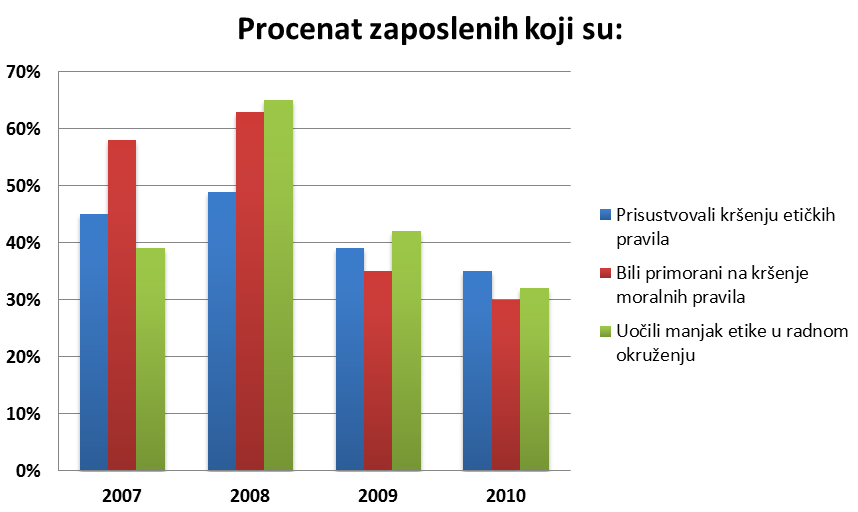
\includegraphics[scale=0.5]{grafik.png}
		\caption{Rezultati ankete u javnim preduzećima}
	\end{center}
\end{figure}
}

%V
\frame{
\begin{itemize}
    \item Motivacija za stvaranje jedinstvenog etičkog i moralnog kodeksa za IT stručnjake. \pause
    \item Poboljšanja koja bi etički kodeks doneo:
\end{itemize}
\pause
\vspace{0.3cm}
\begin{enumerate}
	\item[1.] \textbf{Inspiracija} - Motivacija za informatičare da se ponašaju više u skladu sa etikom.			\pause
		\vspace{0.3cm}
	\item[2.] \textbf{Disciplinovanost} - Doprinos uspostavljanju pravila medu informatičarima.
		\pause
		\vspace{0.3cm}
	\item[3.] \textbf{Informisanost} - Obaveštenje poslodavcima i korisnicima usluga informatičara šta bi 		trebalo i šta bi mogli da očekuju od IT stručnjaka.

\end{enumerate}
}
%----------------------------------------------------------------------------------------
\section{Pravna pitanja u IT svetu}

%VI
\subsection{Elektronska trgovina}
\frame{
\frametitle{Elektronska trgovina}
\begin{itemize}
	\item Autentičnost dokumenata \pause
	\item Pravna nadležnost tokom kupovine \pause
	\item Strah od napredovanja tehnologije; Prednosti i mane
\end{itemize}
}

%VII
\subsection{Zaštita privatnosti i podataka}
\frame{
\frametitle{Zaštita privatnosti i podataka}
\begin{itemize}
	\item Potreba za kontrolisanjem privatnosti i podataka \pause
	\item Organizacija za ekonomsku saradnju i razvoj - \textbf{OECD} \pause
	\item Predlozi zakona OECD-a \pause
	\item Pravila OECD-a
\end{itemize}
}


%VIII
\subsection{Zaštita intelektualne svojine}
\frame{
\frametitle{Zaštita intelektualne svojine}
\begin{itemize}
	\item Problemi kod digitalne intelektualne svojine \pause
	\item \textbf{Copyright}, problemi i prednosti \pause
	\item \textbf{Fair Use}, problemi i prednosti
\end{itemize}
}


%Pozdravni slajd
\frame{
		\begin{itemize}
			\vspace{1cm}
			\item[] \center{{\LARGE Hvala Vam na pažnji!}} \pause
			\vspace{0.5cm}
			\item[] \center{{\Large Pitanja?}}
		\end{itemize}
}

%Poslednji slajd - Literatura
\section{Literatura}
\frame{
\frametitle{Literatura}
		\begin{enumerate}
			\item \textbf{Trust in cyberspace}, Fred B. Schneider, National Academy Press Washington DC

			\item Ethical Issues of Information Technology, Robert G. Wengert, University of Illinois, USA

			\item Ethical issues in an age of information and communication technology, Herman T. Tavani


			\item Beyond the OECD guidelines: Protection of privacy and transborder flows of personal data, Roger Clarke

			\item Copyright or fair use, Joel DuBoff

			\item Legal issues in information security, Joanna Lyn Grama

			\item Property, intellectual property, and free riding, Mark A Lemley
		\end{enumerate}
}
\end{document}
